\documentclass[11pt,a4paper]{article}

\usepackage[margin=1in]{geometry}
\usepackage{amsmath,amssymb,amsthm}
\usepackage{booktabs}
\usepackage{multirow}
\usepackage{graphicx}
\usepackage{microtype}
\usepackage{tikz}
\usetikzlibrary{arrows.meta,positioning,calc,fit,backgrounds,decorations.pathreplacing}
\usepackage{subcaption}
\usepackage[hidelinks]{hyperref}
\usepackage{orcidlink}
\usepackage{natbib}
\bibliographystyle{plainnat}

\newcommand{\bind}{\mathbin{\circledast}}
\newcommand{\unbind}{\mathbin{\oslash}}
\newcommand{\nrm}[1]{\nu\!\left(#1\right)}
\newcommand{\CB}{\mathcal{C}}
\newcommand{\Mem}{\mathcal{M}}

\theoremstyle{plain}
\newtheorem{proposition}{Proposition}
\newtheorem{lemma}{Lemma}
\theoremstyle{definition}
\newtheorem{definition}{Definition}
\theoremstyle{remark}
\newtheorem{remark}{Remark}

\title{One Tick, One Link:\\
{\large A Non-Autoregressive Challenge--Response Memory in Which\\
Depth Is Bought with the World's Silence}}

\author{%
  Xinyu Yang\,\orcidlink{0009-0007-2600-0948}\\
  \href{mailto:Pana.Yang@hotmail.com}{\texttt{Pana.Yang@hotmail.com}}\\
  \href{https://orcid.org/0009-0007-2600-0948}{\texttt{0009-0007-2600-0948}}
}

\date{\today}

\begin{document}
\maketitle

\begin{abstract}
We report a sequence learner that is not autoregressive. It is
\emph{challenge--response}: one input per tick, one output per tick, and
intervals in which the input is the identity and the model keeps emitting. Its
two operations are inverses selected by the world --- speech \emph{binds} an
observation into a superposed store, silence \emph{unbinds} one link out of it
--- so that depth is neither a layer count nor a hyperparameter but the number
of quiet ticks the world grants. Several partial responses mature in parallel
and the one that has matured is said. There is no reward, no label, and no
gradient across a memory write; the only external quantity is prequential
codelength. We verify in isolation that a chain is traversed one link per quiet
tick and halts at its end, derive and confirm the store's operating region
$d>2k\ln V$, show that binding is invertible only for unitary codebooks, and
show that locality-sensitive addressing makes a near miss undetectable by
construction. On a synthetic continual stream retrieval occurs and holds, and
parallel responses are load-bearing. We rule on none of the components that
measure net-negative, because the explanation for all of them rests on a
property of our source rather than of the world, and because a replayed file
cannot test a system for which time is a resource. This version describes the
mechanism as revised since the first write-up (\S\ref{sec:revisions}), and an
appendix records what a real clinical stream and three screened sources taught
it, with the code version behind each result; every experiment there is
open-loop, so none tests the response half of the design.
\end{abstract}

\section{Introduction}

\subsection{Three commitments of the autoregressive frame}

The dominant frame for sequence learning factorises
$p(x_{1:T})=\prod_t p(x_t\mid x_{<t})$, feeds a prefix, and predicts the next
symbol \citep{elman1990finding,vaswani2017attention}. It has been extraordinarily
productive, and it carries three commitments that are easy to stop seeing
because everything around them assumes the same ones.

\paragraph{The objective is next-symbol prediction.} Every metric derived from
it inherits that shape. A system evaluated by per-symbol codelength is being
asked how well it does the thing autoregression is for, whatever else it may
have been built to do.

\paragraph{Computation per symbol is fixed.} A forward pass costs what it costs
whether the world gives the model a microsecond or an hour. Depth is a property
of the architecture, chosen at design time. Recent stateful models
\citep{gu2023mamba} keep a running state rather than a window, but the
computation per token is still fixed and the objective is still next-symbol.

\paragraph{The context is a prefix.} An exact, recent, ordered window.
Long-range association is bought by widening it \citep{beltagy2020longformer,%
dai2019transformerxl} or by retrieving into it \citep{borgeaud2022improving,%
weston2015memory}. Association at distance is thereby made a question about how
much text you can hold, rather than about what you have stored.

For a system meant to run in a real temporal world --- embodied
\citep{brooks1991intelligence}, or agentic over long horizons --- all three sit
badly. There is no prefix boundary in a room. Computation that cannot use extra
time cannot exploit a lull, and lulls are most of what a real stream contains.
And an exact window is the wrong idealisation for a background that in any
organism is a fuzzy, multi-timescale trace rather than a transcript
\citep{brainerd2002fuzzy}.

\subsection{What we put in their place}

We take challenge--response as the primitive. There is no ``a challenge arrives,
now respond'' --- that phrasing is already the autoregressive shape, one prompt
one completion. There is a stream, and every tick carries one input and produces
one output. Some inputs are the world's tokens; in the intervals between them the
input is the identity and the model still emits, iterating on memory. The
model's own emissions are part of its context, interleaved with the world's:
distinguished from them, and combined with them.

The picture we have kept in view is two people talking. While the other is still
speaking you have already begun to think; when they stop, or just as they stop,
you begin to say something. That interval is the gap. What is forming in it is
\emph{not one trajectory} --- several half-formed replies mature together and one
of them is what comes out. Each clause of that sentence turned out to be
load-bearing, and each had to be recovered separately after a run in which the
mechanism measured inert (\S\ref{sec:method}).

The mechanism follows from taking the identity input seriously. If speech means
``there is something to combine'', then silence means ``there is not'', and what
is called for is the inverse operation. Binding writes; unbinding reads; the tick
already says which. Nothing is scheduled, and --- crucially --- nothing needs to
know whether a question is outstanding.

\subsection{What is borrowed}

Storage is content-addressed through a fixed map that no later learning can
move, following the position argued in \citet{yang_2026_22161096}: allocation
buys freedom from interference and pays for it in retrieval difficulty, and the
weakness of the family is that discrimination between addresses decays as
addresses crowd. That trade organises our design, and one of our results is that
in our implementation half of the crowding penalty was self-inflicted
(\S\ref{sec:addressing}).

The representation is holographic \citep{plate1995holographic} in the vector
symbolic tradition \citep{smolensky1990tensor,kanerva1988sparse,%
kanerva2009hyperdimensional,gayler2003vector,eliasmith2013build,%
kleyko2023survey}: binding by circular convolution, reading by circular
correlation, cleanup against a codebook. The pairing of an associative store
with small-world routing follows \citet{watts1998collective}. The readout is a
delta rule \citep{widrow1960adaptive,rosenblatt1958perceptron}. The continual
setting --- regimes arriving, running, departing permanently, with no task
identifier and no boundary signal --- is the one in which catastrophic
interference was characterised \citep{mccloskey1989catastrophic,%
french1999catastrophic} and to which complementary-systems and regularisation
accounts respond \citep{mcclelland1995complementary,kirkpatrick2017overcoming,%
parisi2019continual}.

\subsection{Contributions}

\begin{enumerate}
\item A tick in which binding and unbinding are two halves of one loop selected
by whether the world spoke, so that gap periods, self-output-as-context, and
depth-from-time are consequences of a single rule rather than three mechanisms
(\S\ref{sec:design}, Figure~\ref{fig:tick}).

\item An isolated demonstration that a chain is traversed one link per quiet
tick, halts at its end, and is unharmed by surplus silence
(\S\ref{sec:isolated}, Figure~\ref{fig:walk}).

\item The operating region of a superposed store, $d>2k\ln V$, derived and
confirmed, with the observation that circular correlation inverts convolution
only for unitary codebooks --- a Gaussian codebook loses almost half the signal
with a single item stored (\S\ref{sec:capacity}).

\item A structural result: locality-sensitive addressing makes a near miss
undetectable \emph{by construction}, because a bank's occupants have keys close
to the query. Addressing needs same-content-same-bank and gains nothing from
similar-content-similar-bank (\S\ref{sec:addressing}).

\item An explicit account of what a constructed source cannot settle, and of why
a replayed stream cannot test a model for which time is a resource
(\S\ref{sec:cannot}, \S\ref{sec:limits}).

\item A record of the revisions since the first version, of which version
produced each result, and of what real data taught the design --- including
that every evaluation so far has been open-loop (\S\ref{sec:revisions},
Appendix~\ref{app:empirical}).
\end{enumerate}

\section{Philosophical commitments}
\label{sec:philosophy}

These are not decoration. Each translates into a constraint that the
implementation is checked against, and several of our negative results are
consequences of holding to them.

\subsection{Intelligence as the organisation of memory, not as optimisation
against a scalar}

The founding position of this work is that intelligence is an emergence of
memory rather than a product of reward. The contrast is with the framing in
which behaviour is whatever maximises a scalar
\citep{sutton2018reinforcement,silver2021reward}; here there is no reward, no
value function, and no policy. It is closer to the tradition in which memory is
the computational substrate rather than a subsystem attached to one
\citep{hebb1949organization,tulving1972episodic,gallistel2009memory}.

The design consequence is sharp: the ledger may say what was surprising, and may
therefore decide \emph{what gets written and how deeply}, but it may not be
descended. No gradient crosses a memory write. A node performs a write, not a
fit.

\subsection{Compression as the currency, without frequency as the organiser}

We charge prequential codelength \citep{dawid1984present,rissanen1978modeling,%
blier2018description}, in the tradition that identifies compression with
understanding \citep{solomonoff1964formal,hutter2005universal}. But we
deliberately do not organise memory by frequency, and the reason is a claim
about scale rather than about statistics.

\begin{remark}[Why counts degrade with data]
A per-location count distribution $N(o\mid u)/N(u)$ is a frequency estimate.
As a stream accumulates, the count distribution at any location converges toward
the corpus marginal --- it becomes the global unigram. A counted prior therefore
\emph{stops discriminating exactly as the data grows}: it degrades under
scale, which is the same shape of failure as address crowding.
\end{remark}

More data tends toward disorder; what makes it mean something is organisation,
and organisation need not be a Bayesian prior \citep{jaynes2003probability}.
The delta rule already \emph{is} an organiser of the right kind: it is
error-driven, so a row holds what needed correcting here rather than what was
common here, and a token already predicted stops updating. Counts accumulate and
degrade under growth; the delta rule converges and is stable under it. All
counts and the escape chain were therefore removed, and the graceful degradation
they used to provide was reassigned to the dynamics rather than to a smoothing
rule.

\subsection{An imprecise background is the point, not a compromise}

The background is a fuzzy multi-timescale trace. It is meant to say \emph{which
memories are relevant here}, not to reconstruct what was said. We state as a
non-goal that precise context association is not what this system is for: a
design that makes the background exact has rebuilt the prefix under another
name, and inherits its costs. The nearest cognitive analogue is fuzzy-trace
theory's distinction between verbatim and gist representations
\citep{brainerd2002fuzzy}; the nearest engineering analogue is that a
multi-timescale reservoir is a context, not a transcript
\citep{jaeger2001echo}.

\subsection{Time as a resource, and the ledger that must not be gameable}

If depth is bought with the world's silence, then a system's efficiency is part
of its capability, and evaluation must be conducted where silences are real. A
closely related commitment concerns the shape of the world. If the agent's
actions \emph{generated} its observations, surprise could be minimised by
finding a quiet corner --- the dark-room objection to naive free-energy accounts
\citep{friston2010free,friston2012free,clark2013whatever}. The escape is not a
patch but a property of reality: the world proceeds whether or not the agent
attends, so behaviour \emph{influences} what is experienced without
\emph{generating} it, and missing something costs you later. We return to this
in \S\ref{sec:limits}.

\subsection{Awe, and the limits of a constructed test}

We take seriously that intelligence is not a quantity our source can put under
strain. A constructed stream can isolate mechanisms; it cannot decide whether
those mechanisms amount to anything. We have tried to write the negative results
of \S\ref{sec:cannot} as what they are --- observations consistent with a
plausible mechanism, on a source we argue cannot settle them --- rather than as
verdicts. Where the design should be judged is set out in \S\ref{sec:limits},
and we expect that judgement to be considerably harder than anything reported
here.

\section{Design}
\label{sec:design}

\subsection{Notation and the algebra}

Let $d$ be the width, $\CB=\{E_o\}_{o=1}^{V}\subset\mathbb{R}^d$ the fixed
codebook, $\nu(\cdot)$ normalisation to the unit sphere, and $\bind$ circular
convolution,
\begin{equation}
(a\bind b)_k \;=\; \sum_{j=0}^{d-1} a_j\, b_{(k-j)\bmod d}.
\end{equation}
Write $a^{*}$ for the involution $a^{*}_0=a_0$, $a^{*}_j=a_{d-j}$, and
$m \unbind a \;=\; m \bind a^{*}$ for circular correlation.

\begin{definition}[Unitary codebook]
$a\in\mathbb{R}^d$ is \emph{unitary} if $|\hat a_j|=1$ for every Fourier
coefficient $\hat a_j$. We construct $\CB$ by drawing phases uniformly and
taking an inverse transform, so every $E_o$ is unitary.
\end{definition}

\begin{proposition}[Exact inversion]
\label{prop:inverse}
For unitary $a$, $\;a\bind a^{*}=\delta$, hence $(a\bind b)\unbind a=b$ exactly.
For general $a$, $(a\bind b)\unbind a = b\bind(a\bind a^{*})$, and $a\bind a^{*}$
is a $\delta$ only in expectation.
\end{proposition}

\begin{proof}[Sketch]
Convolution is multiplication in the Fourier domain and the involution conjugates,
so $\widehat{a\bind a^{*}}_j=|\hat a_j|^2$. This is identically one exactly when
$a$ is unitary; for Gaussian $a$ the $|\hat a_j|^2$ are $\chi^2$-distributed with
substantial variance, and the reconstruction is degraded before any interference.
\end{proof}

Proposition~\ref{prop:inverse} is not a technicality. Table~\ref{tab:unitary}
measures the cost: with a \emph{single} triple stored and no interference
whatever, a Gaussian codebook reconstructs at cosine $0.527$.

\subsection{The tick}

\begin{figure}[t]
\centering
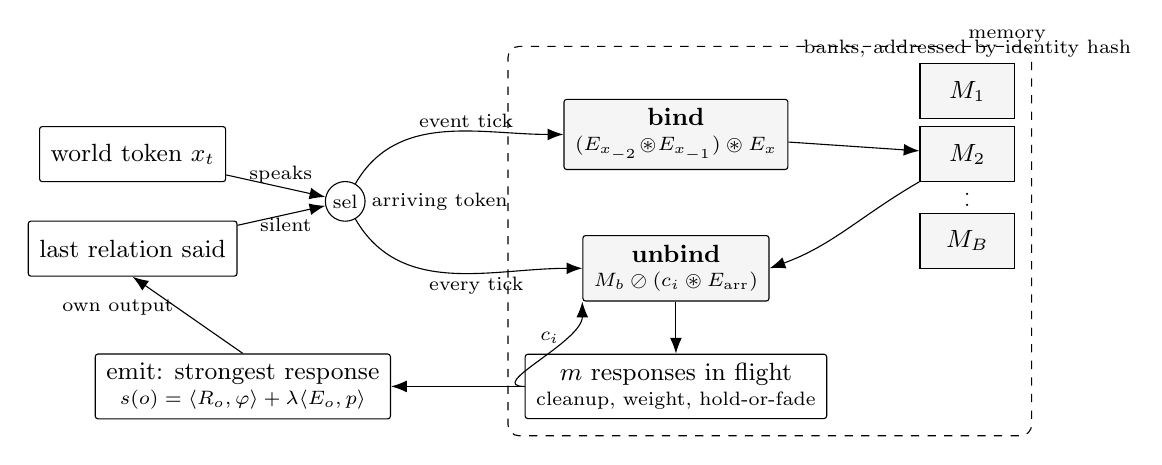
\begin{tikzpicture}[
  font=\small,
  box/.style={draw,rounded corners=1pt,minimum height=7mm,inner xsep=4pt,align=center},
  mem/.style={draw,fill=black!4,minimum height=7mm,minimum width=12mm},
  ar/.style={-{Latex[length=2mm]}},
  lab/.style={font=\scriptsize,inner sep=1pt}
]

\node[box] (world) at (0,3.1) {world token $x_t$};
\node[box] (self)  at (0,1.9) {last relation said};
\node[draw,circle,inner sep=1.5pt] (sel) at (2.7,2.5) {\scriptsize sel};
\draw[ar] (world) -- node[lab,above,pos=.55]{speaks} (sel);
\draw[ar] (self)  -- node[lab,below,pos=.55]{silent} (sel);
\node[lab,right=1pt] at (sel.east) {arriving token};

\node[box,fill=black!4] (bind) at (6.9,3.35) {\textbf{bind}\\[-2pt]
  {\scriptsize $(E_{x_{-2}}\!\bind\! E_{x_{-1}})\bind E_{x}$}};
\node[box,fill=black!4] (unb) at (6.9,1.65) {\textbf{unbind}\\[-2pt]
  {\scriptsize $M_b \unbind (c_i \bind E_{\text{arr}})$}};
\draw[ar] (sel) to[out=60,in=180] node[lab,above,pos=.6]{event tick} (bind);
\draw[ar] (sel) to[out=-60,in=180] node[lab,below,pos=.6]{every tick} (unb);

\node[mem] (m1) at (10.6,3.9) {$M_1$};
\node[mem] (m2) at (10.6,3.1) {$M_2$};
\node[lab]        at (10.6,2.55) {$\vdots$};
\node[mem] (mn) at (10.6,2.0) {$M_B$};
\node[lab,above=1pt of m1] {banks, addressed by identity hash};
\draw[ar] (bind) -- (m2);
\draw[ar] (m2) to[out=-150,in=20] (unb.east);

\node[box] (cur) at (6.9,0.15) {$m$ responses in flight\\[-2pt]
  {\scriptsize cleanup, weight, hold-or-fade}};
\draw[ar] (unb) -- (cur);
\draw[ar] (cur.west) to[out=180,in=-90] node[lab,left,pos=.7]{$c_i$} (unb.south west);

\node[box] (emit) at (1.4,0.15) {emit: strongest response\\[-2pt]
  {\scriptsize $s(o)=\langle R_o,\varphi\rangle+\lambda\langle E_o,p\rangle$}};
\draw[ar] (cur) -- (emit);
\draw[ar] (emit.north) -- node[lab,left,pos=.6]{own output} (self.south);

\begin{scope}[on background layer]
\node[draw,dashed,rounded corners,fit=(bind)(unb)(m1)(mn)(cur),
      inner sep=6pt,label={[lab]above right:{memory}}] {};
\end{scope}
\end{tikzpicture}
\caption{One tick. A token always arrives: the world's when it speaks, the last
relation it said when it does not. Speech binds a triple into the bank named by
the two identities; every tick each response in flight unbinds one link out of
the bank named by its own identity and the arriving one. The emission is the
most matured response, scored by a learned row plus a direct codebook
comparison, and it re-enters as the model's own context. Nothing in the loop
needs to know whether a question is outstanding.}
\label{fig:tick}
\end{figure}

Write $x_{-1},x_{-2}$ for the two previous observed tokens, $c_i$ for the state
of the $i$-th response, $\tau_i$ for the codebook identity it has resolved to,
$w_i\in[0,1]$ for how live it is, and $h(\cdot,\cdot)$ for a hash of two token
identities into $\{1,\dots,B\}$.

\paragraph{Speech binds.}
\begin{equation}
\Mem_{h(\tau_{x_{-2}},\,\tau_{x_{-1}})}
\;\mathrel{+}=\;
\nrm{\big(E_{x_{-2}}\bind E_{x_{-1}}\big)\bind E_{x_t}} .
\label{eq:write}
\end{equation}
For a presented link $x\;r\;y$ the triple formed at the $y$ tick is exactly
$(E_x\bind E_r)\bind E_y$, and no episode boundary was needed to know that. The
sum is \emph{not} renormalised: $\Mem\leftarrow\nu(\Mem+t)$ shrinks everything
already stored by $1/\sqrt2$ per write, giving the first item weight $2^{-k/2}$
--- a sliding window, which is the one thing a superposition must not be.

\paragraph{Silence unbinds; and so does speech.} On \emph{every} tick each
response advances one link:
\begin{align}
q_i &= \nrm{c_i \bind E_{\text{arr}}}, &
r_i &= \nrm{\Mem_{h(\tau_i,\tau_{\text{arr}})} \unbind q_i}, \label{eq:read}\\
\tau_i' &= \arg\max_{o\in\CB_{\text{seen}}} \langle E_o, r_i\rangle, &
c_i &\leftarrow E_{\tau_i'} \ \text{ iff } \
\langle E_{\tau_i'},r_i\rangle > \theta(d,V). \label{eq:cleanup}
\end{align}
Because $\bind$ commutes, a response that has just reached $a_1$ after hearing
$r$ carries $E_{a_1}\bind E_r$ as its next key with no bookkeeping. This is
where the model's own output does its work: the response \emph{is} the position
reached, and the relation stays on the table as the operator.

\paragraph{Arrival holds; speech supersedes.}
\begin{equation}
w_i \leftarrow
\begin{cases}
1 & \text{cleanup accepted},\\
\gamma\, w_i & \text{rejected and the response has never advanced},\\
w_i & \text{rejected and it has advanced at least once (it has \emph{arrived})},
\end{cases}
\label{eq:weight}
\end{equation}
and on every event tick $w_i\leftarrow\gamma w_i$ for all $i$ before a new
response is seeded at the observed token. From inside, ``the chain ended'' and
``the chain never started'' are identical; the only thing separating them is
whether anything was ever retrieved. Holding a half-formed reply while the other
person is quiet, and dropping it when they say something new, is the same
picture.

\paragraph{The emission reads the most matured response.} Let
$i^{\star}=\arg\max_i (w_i, \text{recency}_i)$ lexicographically. Then
$p=c_{i^\star}$, $\varphi=[\,p\,;\,E_x\,;\,\text{bound traces}\,;\,\text{event-locked
bands}\,]$, and
\begin{equation}
s(o) \;=\; \underbrace{\langle R_o,\varphi\rangle}_{\text{learned}}
\;+\;\lambda\underbrace{\langle E_o,p\rangle}_{\text{cleanup}} .
\label{eq:score}
\end{equation}

\begin{remark}[Why not the mixture]
Averaging unit responses and renormalising divides each by
$\|\sum_i w_i c_i\|\approx\sqrt{\sum_i w_i^2}$. Measured, the response holding
the answer arrived at the readout at $0.24$--$0.28$ against a codebook floor of
$0.255$: present and indistinguishable from noise. ``Several half-formed answers
mature together and one of them is said'' is not ``say their average''. Reading
the strongest is the natural readout of parallel responses, not a competition
between mechanisms.
\end{remark}

\paragraph{The event itself.} $E_x$ in $\varphi$ is the lag-zero member of the
family the bound traces form, since $E_x\bind\delta=E_x$; the first version
started at lag one, so a conjunction was present without its parts. Added in
v3 (\S\ref{sec:revisions}): on a stream whose true charge is zero, a new pair
of familiar parts cost $0.408$ bits without it and $0.103$ with it.

\paragraph{The write.} Rows are updated by a delta rule
$R_o \mathrel{+}= \eta\,(\mathbb{1}[o=x]-q(o))\,\varphi$ against the emitted
distribution $q$ --- the distribution the ledger charged. In the first version
(v0) the write reached only the target and the tokens the model ranked
highest, not a uniform sample: correcting what the model would actually have
said. \S\ref{sec:negatives} shows this was the difference between a system
that could represent a non-separable conjunction and one that could not. The
same principle, taken to its limit, weights every token by $q$, and from v2 on
that is what the write does. Truncation had a cost the synthetic source could
not show: on an i.i.d.\ stream, where the right charge for a token of
probability $p$ is exactly $-\log_2 p$, sixteen negatives gave tokens rarer than
$2^{-10}$ a probability near $2^{-50}$, an excess of $41.2$ bits against $0.38$
for the full distribution.

\paragraph{Scoring.} Scores are normalised by subtracting their maximum, not by
clamping them (v1). The delta rule is unregularised and rows grow; once several
scores passed the clamp they became indistinguishable, and on a real stream the
readout charged close to a uniform code ($8.05$ bits against $8.21$). The
cleanup term $\lambda\langle E_o,p\rangle$ ranges over the whole codebook and is
gated separately from the rows (v1): naming a token cannot require that it has
a row.

\subsection{Structural constraints}

Five constraints are asserted by unit tests that run on every build.

\begin{description}
\item[A1 Rate limit.] Constant computation per tick. The only way to think
longer is to occupy more ticks, and ticks are given by the world.
\item[A2 Event-driven accounting.] Charged only when the world speaks, so ``the
identity input injects no new content'' is a consequence of the ledger rather
than an added axiom.
\item[A3 Read/write separation.] The write walk is unperturbed and content
addressed; reads may wander.
\item[A4 No content write at baseline.] Identity ticks write nothing, asserted
bit-for-bit over 500 baseline ticks.
\item[A5 Timescale reachability asymmetry.] The world writes all rungs; the
model's own output reaches only the fastest, so self-generated content
contributes exactly zero to the slow timescales --- a structural ceiling on
confabulation.
\end{description}

\subsection{The background, and why its key is frozen}

The background is a cascaded band-pass ladder: one use of a ladder, on the time
axis only. The memory itself is flat, because a ladder inside the store would be
an abuse of the device.

The bands are snapshotted \emph{at the last event}, so the retrieval key stops
moving when the world does. The reason is that the bands carry two things at
once: which regime this is, which must hold across a silence, and how long the
world has been quiet, which changes every tick. With both in the key, elapsed
time decides whether a memory fires at all --- measured, a fact learned at six
ticks of silence did not answer at one, scoring $0.000$ where the same pair
presented as an ordinary fact scored $0.74$. A clock in the key is a bug; the
live fast rung remains available to the commit rule, which is where elapsed time
belongs.

\subsection{Revisions, and which version a result comes from}
\label{sec:revisions}

The mechanism above is the current one. Table~\ref{tab:versions} lists what
changed since the first version and when. Sections~\ref{sec:isolated}
to~\ref{sec:cannot} were measured on v0 and are reported as they were;
Appendix~\ref{app:empirical} gives the version of every result it reports.

\begin{table}[h]
\centering
\small
\begin{tabular}{llp{9.4cm}}
\toprule
& commit, date & change\\
\midrule
v0 & \texttt{02bdf88}, 09-05 & the mechanism as first written up: top-$k$ negatives, softmax by
clamping, cleanup term inside the readout's gate\\
v1 & \texttt{b96b334}, 09-18 & softmax by subtracting the maximum; cleanup term over the whole
codebook, gated separately from the rows\\
v2 & \texttt{a2b55ee}, 09-18 & the write against the whole emitted distribution\\
v3 & \texttt{a2e3c4a}, 09-20 & the event itself, $E_x$, in $\varphi$\\
v4 & \texttt{433a194}, 09-21 & the read-back check reaches the emission, on by default\\
v5 & \texttt{5ad0013}, 09-27 & cleanup over the codebook rather than over tokens with rows (no
effect while rows are written densely)\\
v6 & 09-28 & read-back check off by default; the switches below documented\\
\bottomrule
\end{tabular}
\caption{Versions of the implementation (all dates 2026).}
\label{tab:versions}
\end{table}

Four mechanisms exist in the code and are \emph{off} by default; each is
documented where it is defined, with its evidence:
\begin{itemize}
\item the read-back check on the emission (above);
\item a gate on the silent walk, built and withdrawn;
\item step-size consolidation rules, measured and not adopted
(Appendix~\ref{app:empirical});
\item an episode trace.
\end{itemize}

The episode trace needs a word, because it touches a commitment. It is a
vector in the volatile state, cleared with the context, into which each event
$x$ is written under the ordered pair of the two events before it. The first
factor of the key is permuted, $i\mapsto 3i \bmod d$, so that the pair is
directional. A key written again has its cleaned old value taken out first. The
recall --- what followed the pair now standing, earlier in this context --- is
named through the codebook with a gain fitted to the charge.

It was built to answer dialogue-state questions (Appendix~\ref{app:empirical}).
It establishes something worth keeping on record: without it nothing in the
situation holds a binding past the bound traces' reach, and the long-term
banks answer ``what did this context bind to $X$'' with the prior. But it is
precise context association, which \S\ref{sec:philosophy} states as a
non-goal, and its gain is a second learner descending the ledger besides the
rows. Whether the design wants that capability is a design question, and until
it is decided the trace stays off.

\section{Isolated verification}
\label{sec:isolated}

\emph{The evidence in this section is from unit tests on synthetic memories in
which every quantity is known. It says what the mechanism does. It says nothing
about whether the mechanism is useful on any data.} We keep the two kinds of
evidence in separate sections throughout, because conflating them is the easiest
way to overstate a result of this kind.

\subsection{One link per quiet tick}

\begin{figure}[h]
\centering
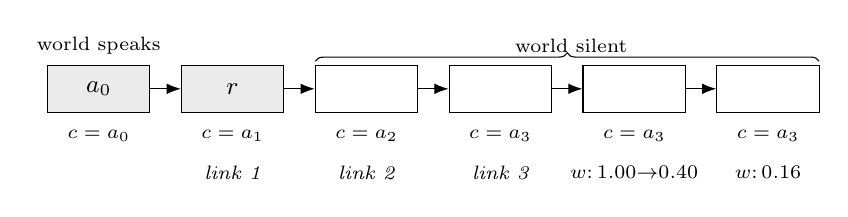
\begin{tikzpicture}[font=\small,
  ar/.style={-{Latex[length=1.8mm]}},
  tk/.style={draw,minimum width=13mm,minimum height=6mm},
  lab/.style={font=\scriptsize}]
\node[tk,fill=black!8] (t0) at (0,0)   {$a_0$};
\node[tk,fill=black!8] (t1) at (1.7,0) {$r$};
\node[tk] (t2) at (3.4,0) {\phantom{x}};
\node[tk] (t3) at (5.1,0) {\phantom{x}};
\node[tk] (t4) at (6.8,0) {\phantom{x}};
\node[tk] (t5) at (8.5,0) {\phantom{x}};
\node[lab] at (0,0.55) {world speaks};
\node[lab] at (6.0,0.55) {world silent};
\draw[decorate,decoration={brace,amplitude=3pt}] (2.75,0.35) -- (9.15,0.35);

\node[lab,below=1mm of t0] {$c=a_0$};
\node[lab,below=1mm of t1] {$c=a_1$};
\node[lab,below=1mm of t2] {$c=a_2$};
\node[lab,below=1mm of t3] {$c=a_3$};
\node[lab,below=1mm of t4] {$c=a_3$};
\node[lab,below=1mm of t5] {$c=a_3$};
\node[lab,below=5.5mm of t1] {\itshape link 1};
\node[lab,below=5.5mm of t2] {\itshape link 2};
\node[lab,below=5.5mm of t3] {\itshape link 3};
\node[lab,below=5.5mm of t4] {$w{:}\,1.00{\to}0.40$};
\node[lab,below=5.5mm of t5] {$w{:}\,0.16$};
\draw[ar] (t0)--(t1); \draw[ar] (t1)--(t2); \draw[ar] (t2)--(t3);
\draw[ar] (t3)--(t4); \draw[ar] (t4)--(t5);
\end{tikzpicture}
\caption{A walk $a_0\!\to\!a_1\!\to\!a_2\!\to\!a_3$ presented forty times among
unrelated traffic, then asked with the start and the relation. One link per
tick; the end of the chain has no outgoing link, so the unbinding returns noise,
cleanup refuses it, and the response holds its answer rather than stepping past
it. Surplus thinking time is harmless. The relation's own response fades on the
same rule.}
\label{fig:walk}
\end{figure}

Four things had to be right simultaneously for Figure~\ref{fig:walk}, and each
was found by a four-second test rather than by an end-to-end run
(\S\ref{sec:method}): the relation is the operator and the model's own output is
the position, not the reverse; seeding must retire the \emph{least live}
response rather than the oldest, because on ties ``oldest'' is the slot holding
the response that has just advanced; responses must be weighted by whether they
are still advancing; and the configuration must lie inside the operating region
below.

\subsection{Capacity, and the operating region}
\label{sec:capacity}

\begin{proposition}[Operating region]
\label{prop:capacity}
Let $\Mem=\sum_{i\le k}t_i$ with $t_i$ unit and mutually near-orthogonal, and
let cleanup take the best match among $V$ codebook entries in $\mathbb{R}^d$.
Then a stored triple returns $\langle\hat\Mem,t_j\rangle\approx k^{-1/2}$, an
unwritten key returns $\approx d^{-1/2}$, and a random vector's best codebook
match is $\approx\sqrt{2\ln V/d}$. Retrieval is usable when
\begin{equation}
\frac{1}{\sqrt{k}} \;>\; \sqrt{\frac{2\ln V}{d}}
\qquad\Longleftrightarrow\qquad
d \;>\; 2k\ln V .
\label{eq:capacity}
\end{equation}
\end{proposition}

At $d=256$ we measure cosine $0.043$ with $k=401$ against a predicted $0.050$.
Equation~\eqref{eq:capacity} is what gives content addressing a job that is not
about accuracy: the address chooses \emph{which} superposition to unbind, each
bank stays under capacity, and the read stays one unbinding however much has
been stored. Related capacity analyses for distributed representations appear in
\citet{plate1995holographic} and \citet{frady2018theory}.

It also fixes the cleanup threshold, which must not be a hand-set constant:
$\theta(d,V)=\kappa\sqrt{2\ln V/d}$. Ours was $0.25$ against a floor of $0.452$
--- \emph{below} the noise --- so cleanup accepted noise on $97.6\%$ of silent
ticks and the response was randomised every tick while the instrument reported
near-perfect success.

\begin{table}[h]
\centering
\begin{tabular}{lccc}
\toprule
codebook & $k=1$ & $k=16$ & $k=64$ \\
\midrule
Gaussian, unit norm & 0.527 & 0.205 & 0.120 \\
unitary (random phase) & \textbf{1.000} & 0.251 & 0.127 \\
$k^{-1/2}$ (theory) & 1.000 & 0.250 & 0.125 \\
\bottomrule
\end{tabular}
\caption{Reconstruction cosine, $d=256$, mean of 12 draws. Proposition~%
\ref{prop:inverse} in numbers: a Gaussian codebook loses almost half the signal
with a \emph{single} item stored, and Proposition~\ref{prop:capacity} is a
statement about unitary vectors. This had been assumed rather than checked for
the life of the project.}
\label{tab:unitary}
\end{table}

\subsection{Addressing must not preserve locality}
\label{sec:addressing}

A key nobody wrote still hashes into an occupied bank, and its occupants answer.
The end of a chain therefore does not retrieve \emph{nothing}; it retrieves a
neighbour. No threshold separates the two, because both are real stored content
of comparable strength. This is address crowding \citep{yang_2026_22161096} in
its sharpest form.

We built a read-back check for it --- bind the candidate back onto the key and
ask whether that triple is in the bank at all --- and it failed instructively.

\begin{lemma}[Locality defeats verification]
\label{lem:lsh}
Under sign-bit locality-sensitive hashing
\citep{indyk1998approximate,charikar2002similarity}, the occupants of a bank
have keys close to the query. If cleanup returns some occupant's target $y_i$
then, for unitary vectors,
\[
\big\langle \nrm{p_i\bind y_i},\ \nrm{q\bind y_i}\big\rangle=\langle p_i,q\rangle,
\]
and $\langle p_i,q\rangle$ being large is \emph{precisely why} $p_i$ and $q$
share a bank. The verification is defeated by the property it was built to
detect.
\end{lemma}

Addressing needs same-content-same-bank and gains nothing from
similar-content-similar-bank; the second property is pure cost and it is what
makes a near miss undetectable. Scrambling the code removes the locality but
makes the address brittle, since write and read reach the same convolution by
different floating-point paths and one flipped sign then means an unrelated
bank. That dilemma is false: cleanup has already resolved the response to an
exact codebook token and the write holds both identities, so the address can be
a hash of the \emph{identities}. Vectors carry the superposition; identities
carry the address. With that in place the read-back check becomes inert --- zero
rejections --- and we report it as doing nothing rather than crediting it.

The check was later wired to the emission (v4): a bound trace whose key the
store reports as never written is zeroed, because what unbinding that address
returns is a neighbour's content. For the pair the model is standing on, the
read-back score separates written from unwritten completely ($0.931$ against
$0.016$, floor $0.088$). It was made the default and returned to off in v6: it
maintains none of the facts of Appendix~\ref{app:empirical}, and its only
support was a snapshot probe on an open-loop prediction benchmark, about one
standard error. It remains a switch.

\section{The source and its instruments}
\label{sec:source}

Regimes arrive, run, and depart permanently; no task identifier, no boundary
signal, no reset. Each carries first-order facts, a Latin square, a product
code, composition chains, and walks. Two families can only be answered by
computing: composition queries are posed \emph{once} per chain and withheld
Latin cells are asked once each, so nothing about them can be memorised from a
previous presentation.

The generator is self-tested before any model is built, because on this project
it produced as many serious defects as the model did.

\begin{table}[h]
\centering
\begin{tabular}{lcc}
\toprule
quantity & Latin square & product code \\
\midrule
$I(T;A\mid D)$, $I(T;B\mid D)$ (bits) & 0.126 / 0.127 & non-zero by design \\
prequential single-cue baseline & 0.201 / 0.195 & 0.486 / 0.402 \\
analytic value & $1/5=0.200$ & $0.500$ \\
composition leakage & \multicolumn{2}{c}{0} \\
facts $\times$ / practice per fact $\times$ at $3\times$ load &
\multicolumn{2}{c}{$2.6$--$3.0$ / $1.00$--$1.14$} \\
\bottomrule
\end{tabular}
\caption{Source self-check, measured on the emitted stream with no threshold.
Marginal information uses the Miller--Madow correction \citep{miller1955note}.
The single-cue baseline is \emph{prequential} --- predict from counts so far,
then update --- because an in-sample ceiling is an oracle that no model charged
before it sees the answer can reach; the in-sample figure is $0.27$ where the
prequential one is $0.20$.}
\label{tab:source}
\end{table}

An earlier version drew one Latin cue from a Zipf distribution and the other
uniformly. For $T=(a+b)\bmod m$, $P(T\mid A)$ is uniform exactly when $p_B$ is,
so that square was \emph{not} zero-marginal: a predictor using cue $B$ alone
reached $0.2745$, and every Latin accuracy the project had reported was at or
below it. Both cues are now uniform, and it must be both --- no choice of square
repairs it, and making both Zipf only makes the leak symmetric. The frequency
skew now lives outside the square, where it forges no shortcut.

\section{End-to-end measurements}
\label{sec:endtoend}

\emph{The evidence in this section is from the full system on the synthetic
stream: 90k ticks, 12 regimes, one seed unless stated. It is source-dependent.}

\subsection{Retrieval occurs, and holds}

\begin{table}[h]
\centering
\begin{tabular}{lcccccc}
\toprule
arm & $t_0$ & $t_1$ & $t_2$ & $t_3$ & $t_4$ & $t_5$ \\
\midrule
control (no superposition) & 0.014 & 0.015 & 0.015 & 0.019 & 0.021 & 0.021 \\
4096 banks, 4 responses & 0.014 & 0.185 & 0.240 & \textbf{0.268} & 0.237 & 0.238 \\
8192 banks, 4 responses & 0.014 & 0.189 & 0.243 & \textbf{0.275} & 0.248 & 0.250 \\
4096 banks, \emph{1} response & 0.006 & 0.193 & 0.007 & 0.010 & 0.013 & 0.013 \\
\bottomrule
\end{tabular}
\caption{Cosine between the emitted response state and the correct answer, by
tick of silence; $t_0$ is the relation's own tick. Retrieval happens and holds.
With a single trajectory it happens and then collapses --- the cleanest evidence
we have for the ``not just one trajectory'' clause.}
\label{tab:cursor}
\end{table}

\subsection{Competitive negatives}
\label{sec:negatives}

The largest single effect we measured was not a design choice but the repair of
a defect. The delta rule drew negatives uniformly from every known token.
Discrimination on a Latin item rests entirely on pushing down the five rivals
sharing a square's six targets; each was drawn about $2.3\%$ of the time against
a target appearing roughly eighteen times in a regime's life, so a rival
received a negative gradient about $0.4$ times. The readout was never taught to
separate the six and settled at $1/6$ --- and, because the product code is
answerable from marginals where positive-only ranking suffices, the
separable/non-separable split that had organised months of analysis was a
property of the sampler rather than of the architecture.

\begin{table}[h]
\centering
\begin{tabular}{lcccc}
\toprule
negatives & Latin & product & one-shot composition & answer bits \\
\midrule
uniform, $k{=}16$ & 0.1448 & 0.6884 & 0.0150 & 6.249 \\
uniform, $k{=}64$ & 0.2421 & 0.7612 & 0.0150 & 5.173 \\
top-$k$, $k{=}16$ & \textbf{0.4529} & \textbf{0.8426} & \textbf{0.3308} & \textbf{3.970} \\
top-$k$, $k{=}64$ & 0.4444 & 0.8426 & 0.3459 & 3.984 \\
\bottomrule
\end{tabular}
\caption{Correcting what the model would actually have said rather than random
tokens \citep{mikolov2013distributed}. Raising the uniform count moves the same
way and falls well short, which is the control saying this is about \emph{which}
negatives and not how many. Composition goes from zero to a third: chaining two
stored facts was not absent, it was unreachable.}
\label{tab:negatives}
\end{table}

\subsection{Exposure, and what it says about sources of this shape}

\begin{table}[h]
\centering
\begin{tabular}{lcccc}
\toprule
family & 1st exposure & 2nd & 3rd & 4th+ \\
\midrule
Latin ($n=286$ firsts) & 0.000 & 0.03 & 0.33 & 0.87 \\
product ($n=72$)       & 0.000 & 0.02 & 0.37 & 0.995 \\
composition ($n=35$)   & 0.000 & 0.00 & 0.23 & 0.95 \\
\bottomrule
\end{tabular}
\caption{Accuracy by how many times a fact had already been charged, under an
earlier configuration. Every family is exactly zero the first time and near
ceiling by the fourth: every aggregate on a present--repeat--ask source is
carried by re-lookup. This is why composition queries and withheld cells are now
asked \emph{once}.}
\label{tab:exposure}
\end{table}

Table~\ref{tab:exposure} also exposes a representational fact. A novel product
pair scores $0.000$ where cue $A$ alone would give $0.5$: $E_a\bind E_b$ is a
lookup key, not a decomposable representation, so an unseen combination is a
fresh random vector uncorrelated with anything stored. We have the
\emph{combine} half of distinguish-and-combine, and a learned linear readout
cannot recover the parts. That is exactly the gap the unbinding half of
\S\ref{sec:design} exists to close, and closing it is what moved composition from
$0.015$ to $0.331$ in Table~\ref{tab:negatives}.

\subsection{Aggregates}

\begin{table}[h]
\centering
\small
\begin{tabular}{lccccc}
\toprule
arm & Latin & product & retention & answer bits & walk support \\
\midrule
no superposition        & 0.5695 & 0.8273 & 0.4187 & 3.141 & 0.517 \\
baseline                & 0.6090 & 0.8290 & 0.4405 & 3.060 & 0.546 \\
banks $=1$              & 0.5679 & 0.8282 & 0.4464 & 3.051 & 0.540 \\
banks $=65536$          & 0.6107 & 0.8290 & 0.4306 & 3.056 & 0.546 \\
\midrule
bind off \emph{(must collapse)} & 0.1809 & 0.7029 & 0.2996 & 4.577 & 0.219 \\
\bottomrule
\end{tabular}
\caption{Single seed; codelength charged at the answer tick only. Against the
single-cue baselines of Table~\ref{tab:source} ($0.20$ and $0.49$) both
conjunction families are answered well above a predictor that ignores half the
challenge. The collapse arm holds, which is what makes the rest readable.}
\label{tab:endtoend}
\end{table}

\section{What this source cannot settle}
\label{sec:cannot}

Three components measure net-negative here: the ladder feedback of the model's
own channels, the operator graph, and background depth beyond one rung. One
mechanism explains all three and the arms order monotonically by it. We rule on
none of them.

\begin{table}[h]
\centering
\small
\begin{tabular}{lccccl}
\toprule
arm & Latin & retention & answer bits & walk $d{=}1$ & non-fact content in $\varphi$ \\
\midrule
all streams off  & 0.6147 & 0.4802 & \textbf{2.943} & [.286 .222 .667 .200] & least \\
baseline         & 0.6090 & 0.4405 & 3.060 & [.000 .111 .333 .000] & \\
live bands       & 0.6123 & 0.4008 & 3.138 & [.000 .000 .333 .000] & $+$ a clock \\
graph re-enabled & 0.5913 & \textbf{0.3413} & \textbf{3.428} & [.000 .000 .333 .000] & most \\
\midrule
rungs $=1$       & 0.5751 & \textbf{0.6111} & 3.359 & [.286 .000 .333 .200] & fewest bands \\
rungs $=5$       & 0.5775 & 0.4702 & \textbf{2.948} & [.000 .222 .333 .200] & most bands \\
\bottomrule
\end{tabular}
\caption{Single seed. Retention age-decay slopes: $-0.023$ at one rung against
$-0.072$ at the baseline's three. Walk cells hold six to nine events and are not
a strong result.}
\label{tab:cannot}
\end{table}

\paragraph{The hypothesis.} $\varphi$ is a fixed-width retrieval key. Anything
added to it that is not a function of the fact being asked about adds variance
without signal. On this source a Latin answer is determined by its two cues, so
what the model just said carries no information about it while making $\varphi$
differ between two presentations of the same fact. The operator graph is
near-random for the same reason its learning does nothing: each edge receives
ten to forty rank-one updates against $4096$ parameters, and its drift grows as
$\sqrt{\text{updates}}$ --- the signature of uncorrelated accumulation. Bands are
context, not fact.

\paragraph{Why we do not rule.} Every one of these rests on the source's answers
being cue-determined, which is the property of a constructed source most open to
doubt. The hypothesis predicts a sign flip on a source where the answer is
\emph{not} cue-determined and the model's own trajectory carries necessary
information; the only family here with that property has cells of six to nine
events.

\paragraph{The three-stream requirement has two implementations with opposite
signs.} Ladder feedback carries no signal here and is net-negative. Cursor
advance --- the model's own output as the position a chain has reached --- is
load-bearing (Table~\ref{tab:cursor}). The founding requirement that input and
output streams interleave as context is met by the second; the first is one way
of writing it that happens to hurt here. Reporting them as a single verdict
would be wrong.

\paragraph{A test we abandoned.} We proposed measuring the variance of $\varphi$
across repeated presentations of the same fact. It has almost no power: $2304$
dimensions, four to nine presentations per fact, and a rank correlation between
two noisy orderings. Two difference tests replace it --- excluding a component
from $\varphi$ while leaving it in the dynamics, and substituting a noise block
of matched width and variability --- but both belong on real data
(\S\ref{sec:limits}).

\section{Method: five failures of one shape}
\label{sec:method}

\begin{table}[h]
\centering
\small
\begin{tabular}{p{4.2cm}p{5.6cm}p{4.1cm}}
\toprule
symptom & cause & what found it \\
\midrule
self-stream ablation reads zero & feature blocks wider than rows; three
background bands silently truncated & per-block alignment assertion \\
near-miss curve flat & the write path was dead code; reads and writes landed on
the same perturbed edge & call-graph grep \\
every accuracy collapses & a decay constant applied \emph{per tick}, leaving
$1.6\%$ of the binding by the time it was read & the mechanism's own off-control \\
six arms bit-identical & the retrieval never reached the emission & the
bit-identity itself \\
cleanup succeeds $97.6\%$ and is always wrong & the threshold sat \emph{below}
the codebook noise floor ($0.25$ against $0.452$) & measuring four numbers
directly \\
\bottomrule
\end{tabular}
\caption{Each symptom reads as ``a mechanism measures inert''. Each cause is
that the mechanism's product had no outlet, or was erased downstream.}
\label{tab:failures}
\end{table}

The discipline this forces, stated because we expect it to generalise to any
system of this shape:

\begin{enumerate}
\item Any change on the path of a load-bearing mechanism gets that mechanism's
off-control \emph{in the same sitting}. If the full arm and the off arm are
close, stop.
\item A terminal metric cannot debug a multi-step chain. An end-to-end zero has
no power to say which of five steps broke: four-second unit tests found four
errors where ten-minute end-to-end runs found none.
\item Bit-identical arms are more alarming than bad numbers.
\item Any hand-set constant must be back-solved from its own units. Three of our
failures were constants never checked against the scale they operate on.
\item Suspect the data before the mechanism.
\end{enumerate}

Performance belongs in the same list, because where computation is bought with
the world's time it is not merely engineering. Replacing an address that
regenerated $4096$ random keys per call with pre-generated sign bits took one
arm from over twenty-one minutes to $6$m$43$s, and the $O(d^2)$ convolution
became $O(d\log d)$, which is also what makes the unitary codebook affordable.

\section{Limitations, and what a real evaluation requires}
\label{sec:limits}

\paragraph{A replayed stream cannot test a model for which time is a resource.}
Our silences are drawn from $\{1,2,4,8\}$ --- authored, not observed. The model
is never late: it receives exactly the ticks the file specifies regardless of
how much computation it needed. There is no rate, and in a real continual
setting the ratio between the world's event rate and the agent's compute rate is
decisive. Replay tests mechanism; it cannot test the claim this architecture
exists for.

\paragraph{The autoregressive baseline is the wrong yardstick and the right
lower bound.} We report PPM \citep{cleary1984data} not as a standard to beat ---
that adopts the next-symbol objective as the measure --- but as a control that
\emph{cannot accumulate}: a bounded window carries nothing across itself, so a
sustained gap is evidence of accumulation. On charged events, order-4 PPM costs
$11.80$ bits at accuracy $0.008$ and scores exactly $0.000$ on both conjunction
families, against $9.17$ bits and $0.206/0.732$ for the mechanism at the time of
that comparison. The variant handed the segmentation the mechanism refuses to
assume reaches $5.60$ bits, and losing to that is the comparison worth losing.

\paragraph{Our source has no transferable structure.} Each regime carries its own
square, entities and product code and shares nothing with any other, so transfer
is impossible by construction and an acquisition-acceleration measurement --- is
the $n$-th regime learned faster than the first? --- is guaranteed flat. If a
constructed source is retained, the one change worth making first is shared
latent relations across regimes, because that is the minimum condition under
which organisation has anything to organise.

\paragraph{Attention is empty without laws.} Letting the model's state influence
which of the concurrently live regimes speaks next --- $P\propto
\exp(\beta\cdot\text{align})$, with $\beta=0$ recovering the present source
exactly --- is meaningful only when the same regularity recurs across
situations, so that attending here teaches you about there. The world's
progression must remain exogenous: things happen whether or not the agent
attends, and that property alone stops the ledger being gamed by an agent that
finds a quiet corner \citep{friston2012free}. Real reactions are influenced by
the individual without being generated by it, and requiring a full self-loop is
the wrong route.

\paragraph{No evaluation here is closed-loop.} Neither the synthetic source nor
any real source of Appendix~\ref{app:empirical} lets the model's output change
what the world does next: $\beta$ above has stayed at zero. Every result in this
paper is therefore about memory and prediction. The response half of
challenge--response --- what is said, and what the world does because it was
said --- has not been tested at all, and a world in which behaviour influences
experience without generating it is the evaluation this design most needs.

\paragraph{What would settle these questions.} Real language content carrying
real, non-authored temporal structure: timestamped transcripts, subtitle
streams, conversation logs --- data in which silences are real silences of real
duration and the two-people-talking picture is the data rather than an analogy.
A tick then corresponds to a unit of real time, and the natural next step binds
the compute budget to wall-clock, at which point depth-from-time becomes a
genuine constraint and the efficiency of an implementation becomes part of its
capability. This is where \citet{lecun2022path} and the embodied tradition
\citep{brooks1991intelligence,clark2013whatever} both point.

\paragraph{Caution.} We do not know what these mechanisms do on real data and do
not think it can be predicted from here. Every result is single-seed unless
stated, and the families that cannot be memorised carry sixty to ninety-six
events in total.

\section{Related work}

\paragraph{Distributed binding.} Our store is a superposition read by
correlation, in the holographic \citep{plate1995holographic} and tensor-product
\citep{smolensky1990tensor} traditions, addressed the way sparse distributed
memory addresses \citep{kanerva1988sparse}, and surveyed as hyperdimensional
computing \citep{kanerva2009hyperdimensional,gayler2003vector,%
eliasmith2013build,kleyko2023survey}. Capacity of such stores is analysed by
\citet{plate1995holographic} and \citet{frady2018theory}; our
Proposition~\ref{prop:capacity} is the form we needed, coupling capacity to a
cleanup codebook of size $V$. Classical associative memories
\citep{willshaw1969non,hopfield1982neural,kohonen1972correlation} are the
ancestors of the readout.

\paragraph{Learned versus fixed addressing.} Differentiable memories
\citep{graves2014neural,graves2016hybrid,weston2015memory} and modern
associative layers \citep{ramsauer2021hopfield} learn where things go. Ours is
fixed by construction, following \citet{yang_2026_22161096}: an address that no
later learning can move is what buys freedom from interference, and the price is
retrieval difficulty. Fast-weight schemes
\citep{schmidhuber1992learning,ba2016using} also write associations at inference
time, but inside an autoregressive objective.

\paragraph{Random transforms.} The graph component turned out to behave as a
random feature expansion \citep{rahimi2007random} feeding a linear readout,
which is the regime reservoir computing occupies deliberately
\citep{jaeger2001echo,maass2002real}. We report this as a negative structural
finding rather than as a design.

\paragraph{Continual learning.} The setting and its interference are classical
\citep{mccloskey1989catastrophic,french1999catastrophic}; responses include
regularisation \citep{kirkpatrick2017overcoming}, replay
\citep{lopez2017gradient}, and architectural allocation, surveyed by
\citet{parisi2019continual}. Our position is the allocation one, taken to its
committed form.

\paragraph{Compression and prediction.} The ledger is prequential
\citep{dawid1984present,rissanen1978modeling} in the description-length reading
of learning \citep{blier2018description,grunwald2007mdl}, and the identification
of compression with understanding is argued at length by
\citet{solomonoff1964formal} and \citet{hutter2005universal}. What we do not
take is the objective: there is no reward here
\citep{sutton2018reinforcement,silver2021reward}.

\paragraph{Autoregressive systems can do these tasks.} A long-context model can
solve retrieval of this shape by induction \citep{olsson2022context}, and
state-space models \citep{gu2023mamba} carry a running state rather than a
window. Neither can spend a lull: computation per token is fixed, and that is
the axis on which this work differs.

\section{Conclusion}

We built a challenge--response memory in which binding and unbinding are the two
halves of one tick, selected by whether the world spoke, and in which several
partial responses mature in parallel while the world is quiet. In isolation the
mechanism does what the design says: one link per quiet tick, a halt at the end
of a chain, surplus silence harmless. We derived the operating region of its
store, showed that binding inverts exactly only for unitary codebooks, and
showed that locality-sensitive addressing makes a near miss undetectable by
construction --- so half of the crowding penalty this family is known for was,
in our implementation, self-inflicted.

On a synthetic continual stream retrieval occurs, holds, and requires several
trajectories rather than one. Several components measure net-negative with one
mechanism that explains them; we rule on none, because the explanation rests on
a property of the source rather than of the world, and because a replayed file
cannot test a system for which time is a resource. What we claim is feasibility
at this scale on this source, for a design that is non-autoregressive at its
root, that treats precise context association as a non-goal, and that is aimed
at stateful continual learning in a world that has a clock. Where it should be
judged is on real language carrying real time, and we expect that judgement to
be substantially harder than anything reported here.

\subsection*{Reproducibility}

At v6 the implementation is $19{,}377$ lines of Rust with no dependencies,
deterministic under a counter-based generator with fixed-order float
reductions, carrying $36$ structural assertions and $6$ generator self-tests
that run on every build (at v0: $8953$ lines, $20$ assertions). Two
identical runs agree bit-for-bit. Constraints A1--A5 and each mechanism claim of
\S\ref{sec:isolated} are asserted by a named test.

\appendix

\section{An empirical case: intensive-care streams, and three screened sources}
\label{app:empirical}

This appendix was added after the body of the paper and records what one real
dataset taught the design. It is not a benchmark claim. Figures are from a
single seed; where the number of positives is small the standard error is
stated. Every figure was checked against a saved run output or re-run; where a
figure could not be recovered it is stated qualitatively. Each carries the
version of the code that produced it (Table~\ref{tab:versions} in
\S\ref{sec:revisions}, and Table~\ref{tab:provenance} below).

\paragraph{What is not tested.} Every experiment below is \emph{open-loop}: the
world's next event is fixed in advance and does not depend on what the model
said. The questions are answered by the world whatever the model answered. They
therefore test memory and prediction, and not the response half of
challenge--response. The circumstance ``what was asked before'' is never
produced by the learner's own answers. The design calls for a world whose
progression the learner's behaviour influences without generating it
(\S\ref{sec:philosophy}, \S\ref{sec:limits}), and no experiment here has one.

\begin{table}[h]
\centering
\small
\begin{tabular}{p{8.4cm}cp{3.6cm}}
\toprule
result & version & note\\
\midrule
timing alone, SAPS-I, SOFA; Electricity; panel information; PPM's use of the
gap; the three screens & --- & no model involved\\
probe table and the $+0.025$ of two mechanisms & v4 & the off arm is v2
without the self block\\
bedside table; step $0.02$ at the bedside; horizon $2048$ & v4 & \\
codelength $3.379$ and the association table (all stays); the gate on the
silent walk & v4 & \\
association table on the first 400 stays; subset trend & v4 & working tree of
\texttt{433a194}\\
transfer across pools; replay & v4 & \\
rarity excess ($41.2$ against $0.38$ bits) & v5 & re-run\\
noisy-label table & v5 & re-run\\
dilution; proper scores on the synthetic judge & v4 & \\
descent against floor; step rules & v4 & working tree of \texttt{433a194}\\
MultiWOZ with and without the episode trace & v6 & trace switched on\\
facts matrix & v6 & re-run\\
the early full-stream run near a uniform code & v0 & reported as the defect
it exposed\\
\bottomrule
\end{tabular}
\caption{Which code version produced which result of this appendix.}
\label{tab:provenance}
\end{table}

Two results measured on v0 during this work are not reported: the value of
silence to the memory on the clinical stream ($0.14$--$0.26$ bits per event),
and the share of the gap the memory took against PPM ($0.169$ against $0.180$
bits). Both were produced by the emission path that v1 repaired, and neither
has been re-measured.

\subsection{Data, and why this source}

PhysioNet/CinC Challenge 2012 \citep{silva2012predicting}, set-a: 3996
intensive-care stays, 1.73M timestamped measurements. Each measurement is one
token (parameter, octile of its value), $V=296$. Elapsed time between
measurements enters as idle ticks, $\lfloor\log_2\rfloor$ of the gap in minutes,
capped at 11. In-hospital death: 554 stays (13.9\%).

The source was chosen by a screen of its own. Standard concept-drift streams
fail one. Electricity is sampled every thirty minutes without exception
(coefficient of variation of the gaps $0.000$), and predicting the previous
label scores 0.853 against 0.752 for naive Bayes, so the benchmark cannot show
anything about a memory. Irregularly sampled clinical series are the opposite
case: the observation times carry information. Using only \emph{when}
measurements were taken and never their values, in-hospital death is predicted
at AUROC 0.616 (the number of measurements in the last six hours), against
0.637 for SAPS-I and 0.626 for SOFA, which are computed from the values.

\subsection{A prediction at one position is not a relational question}

In-hospital death is fixed at one position, the end of the stay, and it is a
function of an order-free summary of the whole stay. Under a five-fold
cross-validated linear probe (AUROC; memory v4):

\begin{center}
\small
\begin{tabular}{lc}
\toprule
representation & AUROC\\
\midrule
count and mean-gap summary of the whole stay & 0.803\\
memory state, max-pooled over the stay & 0.784\\
memory state, mean-pooled & 0.774\\
count summary plus hashed bigrams & 0.770\\
hashed bigrams alone & 0.750\\
memory state at the final tick & 0.713\\
SAPS-I score & 0.635\\
timing alone, best single feature & 0.616\\
\bottomrule
\end{tabular}
\end{center}

Adding bigrams to the count summary lowers it, from 0.803 to 0.770: order
carries nothing here beyond counts. Two mechanisms, the lag-zero self block
(v3) and the read-back check (v4, off by default since v6), raise the
max-pooled readout by $0.025$ (mean-pooled by $0.017$). They lower the
final-tick readout from 0.727 to 0.713: what they add helps the trajectory, not
the snapshot at its end. The label is terminal structure, and an evaluation
that can be redone at any time sees nothing that depends on position.

The same question was then asked in the architecture's own shape (v4). The
outcome is an event the world speaks at the end of the stay. Memory is
continual across stays; the first half of the stays are learned from and the
second half read. During a stay the question is put as a frozen probe at a
quarter, a half and three quarters of the way through:

\begin{center}
\small
\begin{tabular}{lcccc}
\toprule
asked at & memory & memory, stay wiped & counter, online & counter, batch\\
\midrule
25\% & 0.584 & 0.493 & 0.741 & 0.751\\
50\% & 0.651 & 0.493 & 0.765 & 0.764\\
75\% & 0.666 & 0.493 & 0.775 & 0.781\\
end & 0.701 & 0.493 & 0.794 & 0.796\\
\bottomrule
\end{tabular}
\end{center}

The end-of-stay figure is close to the final-tick probe (0.701 against 0.713).
The two protocols differ (a prequential half split against five-fold
cross-validation) and are not strictly comparable. The closeness suggests that
the readout takes out of the present state about what a linear probe does, and
that what the present state lacks is the whole stay: the slowest background
band spans 256 ticks, while a stay averages about 640.

Lengthening that band to 2048 ticks tests this, and supports it only in part:
\begin{itemize}
\item the end-of-stay AUROC rises from 0.701 to 0.721 (0.605 at a quarter of
the stay, from 0.584);
\item the final-tick probe rises from 0.713 to 0.731;
\item the mean-pooled probe is unchanged (0.774), and the max-pooled one falls
(0.784 to 0.746);
\item the gap to the online counter at the end of the stay narrows only from
0.093 to 0.073.
\end{itemize}
A memory whose state is recency-weighted holds a whole-history count only in
part, and a longer horizon alone does not make it one.

\subsection{Screening a source before the model sees it}

If last-$k$ events, counts, or counts with elapsed time already answer a
question, no state can show anything on that question, however good it is.
Three sources were screened (accuracy of memoryless judges on held-out cases):

\begin{itemize}
\item \emph{PhysioNet mortality}: the order-free count summary reaches 0.80,
and adding order lowers it; unsuitable for showing a memory of order.

\item \emph{BPI Challenge 2012} \citep{vandongen2012bpi}, a loan-application
process log, 13087 cases. Structural questions about the case so far (``has an
offer been sent'', ``is the latest offer event a cancellation'') are answered at
$\ge0.95$ by the last two events or by counts. Questions about elapsed time
leave room (``over 7 days since the offer was sent'': counts with elapsed time
0.897), but they reduce to keeping a clock. Unsuitable.

\item \emph{MultiWOZ~2.2} \citep{budzianowski2018multiwoz,zang2020multiwoz},
10437 task-oriented dialogues, about $6\times10^5$ questions ``what value does
the user currently want for slot $s$'', asked after every user turn. The rule
``the last value the user gave for $s$'' answers 0.908, and restricting it costs
0.23--0.33:
  \begin{itemize}
  \item the same rule over the last three turn pairs only, 0.677;
  \item the most frequently mentioned value, 0.579;
  \item the last value mentioned by either speaker, 0.582.
  \end{itemize}
The source passes the screen, and it is still unsuitable for this design.
About nine questions in ten are literal: the answer is a value the user said,
and a dictionary keyed by speaker, domain and slot answers them at 0.99, so no
memory can do better than match it there. The remainder, mostly an offer
accepted with ``yes'', is where organisation could show.

With the episode trace of \S\ref{sec:revisions} switched on (v6; 1000
dialogues, $d=512$):
  \begin{itemize}
  \item overall, 0.525 without the trace against 0.619 with it;
  \item for a value said in the same turn, 0.512 against 0.789;
  \item where the user never gave the value, 0.21 either way, against 0.51
  for the best rule.
  \end{itemize}
It helped only where the answer was a recent literal, which is the part a
dictionary already answers.
\end{itemize}

\subsection{The unit of prediction decides what is measured}

At the granularity of a panel (the set of parameters recorded at one time) the
stream appeared to hold an opening. The gap carries
$I(\text{panel};\text{gap}\mid\text{previous panel})=0.485$ bits (a plug-in
estimate), 10\% of the conditional entropy. Yet conditioning PPM's order-3
context on the gap \emph{cost} it 0.047 bits per event, because 3600 distinct
panels fragment every context it needs.

At the granularity of a single parameter ($V=37$, measured on 600 stays) this
inverts: PPM takes the gap, from 1.215 to 1.035 bits per event. The opening was
a property of a bad prediction unit, not of the source. The choice of
individuation is part of the question, and an advantage that appears under one
individuation and not under a better-posed one is not an advantage of the
learner.

\subsection{Codelength is an instrument, not an objective}

Next-token codelength (v4) against PPM \citep{cleary1984data} at its best order
(order 2) over the same stream: 3.379 bits per event against 4.097. This is the
reading \S\ref{sec:limits} calls the wrong yardstick and the right lower bound,
and it is reported as such.

Take the events whose order-2 context is new but whose order-1 context is not.
There the margin depends on how often the (order-1 context, target)
association had been seen before:
\begin{itemize}
\item never: $+2.74$ bits;
\item once: $-1.03$;
\item two to four times: $-0.95$;
\item five to nineteen: $-0.26$;
\item twenty or more: $+0.08$.
\end{itemize}
On the first 400 stays alone the same cell reads $+2.43$, $-1.91$, $-1.61$,
$-0.45$, $+0.37$: the shape holds and the negative band narrows with
experience. A counter holds an association after one occurrence; the delta rule
needs several corrections. That band is a rate, not a price: it is where the
memory has not yet arrived.

Two earlier readings of the same column were wrong in instructive ways.
\begin{itemize}
\item \emph{Composition or rarity.} The loss on new contexts first looked like
a failure to compose. Split by the rarity of the target, most of it was
rarity. For targets seen a hundred times or more, new contexts are ahead of PPM
as seen ones are ($+0.29$ and $+0.52$ bits, against $+0.44$ and $+0.77$). The
losses concentrate on targets seen one to ninety-nine times ($-0.65$, $-0.60$).
At matched rarity a new context still costs 0.15--0.75 bits more than a seen
one, so rarity is the larger part of the loss, not all of it. The rarity loss
was the truncated write of v0--v1, which v2 replaced (\S\ref{sec:design}).

\item \emph{A trend on a subset.} On 400 stays both columns appeared to
improve steadily through the stream; on all 3996 they settle by the second
decile. 175k events lie entirely inside the learning phase, so a trend read
there describes the subset.
\end{itemize}

Two findings limit what the number can say:
\begin{itemize}
\item \emph{It does not separate organisation from counting.} Take 400 patients
from a set never seen, and pools of 200 to 3200 patients from the other set
(v4).
  \begin{itemize}
  \item One pass over a pool lowers the codelength on the unseen patients by
  about 0.045 bits per doubling of the pool, without saturating. PPM falls at
  the same rate, and the margin stays flat at $0.74$--$0.76$.
  \item Past one pass over the same pool, both absolute codelengths worsen
  while the margin widens. The absolute column, not the margin, is the one to
  read.
  \end{itemize}

\item \emph{A gain without a mechanism is not a reason to adopt.} A gate that
refuses a silent hop collapsing onto the token just heard (v4, never adopted)
improved the codelength by 0.046 bits overall and by 0.124 bits on events in
new contexts. The explanation offered for the gain was tested and not
supported, so the gate was not adopted. The test applied was: would this change
still be right if the charge got worse? The read-back check is the same case in
the other direction: made the default on an argument in v4, and returned to off
in v6 because its measured support was a benchmark of the wrong kind.
\end{itemize}

\subsection{Noise floors depend on whether the target is noisy}

A fixed-step least-mean-squares readout has a steady-state misadjustment
proportional to the step and to the noise on the target, and none on a
deterministic target \citep{widrow1960adaptive}. This was checked on a question
with a known ceiling (v5): the spoken answer is flipped with probability 0.2, so
the best AUROC is exactly 0.800 and the best Brier score exactly 0.160.

\begin{center}
\small
\begin{tabular}{cccc}
\toprule
step & AUROC & Brier & ECE\\
\midrule
0.2 & 0.773 & 0.206 & 0.110\\
0.05 & 0.797 & 0.178 & 0.072\\
0.02 & 0.801 & 0.169 & 0.057\\
0.005 & 0.807 & 0.175 & 0.059\\
\bottomrule
\end{tabular}
\end{center}

The alternative, that the answer is simply too rare to learn, was rejected.
With the question held easy, accuracy stays at 0.999--1.000 as the answer grows
rarer, down to one answer in 514 events.

On the clinical stream (v4) the step of 0.02 fixed calibration, not
discrimination. The charge on the spoken outcome fell from 0.627 bits, above the
base-rate entropy of 0.590, to 0.586, and answers stopped changing during the
silence. AUROC moved only from 0.701 to 0.712.

The converse error was also made (v4). A residual on a stationary deterministic
stream was first read as this misadjustment. A sweep refused it:
\begin{itemize}
\item the residual \emph{shrank} as the step grew (0.085 at step 0.5, 0.238 at
0.05, measured after $10^5$ events), whereas a misadjustment grows with the
step;
\item recovery after a change was slower at the smaller step too (6236 against
11483 events);
\item on a stationary stream of $6\times10^5$ events, the residual at steps
0.2 and 0.05 was still falling in the last segment (0.044 to 0.043, and 0.099
to 0.091). Only at step 0.5 had it levelled.
\end{itemize}
It was a descent in progress, not a floor.

Two step rules that shrink the step as a row settles were measured on a stream
whose map is replaced halfway:
\begin{itemize}
\item a step of $\eta/(1+n)$ never learns: 5.4 bits, against 1.1 for the fixed
step, in the first segment;
\item an error-driven step recovers as well as it learns, but converges an
order of magnitude worse: 0.90 against 0.11.
\end{itemize}
Neither can tell ``the error is small because this row has learned'' from ``the
error is small because it is nearly there''.

Next-token structure on the same stream prefers the larger step, so one global
step cannot serve both. Separating ``learning structure'' from ``chasing noise''
requires a quantity other than the error: on a noisy target the error never
falls. Which quantity, without reintroducing a scalar objective, is open.

\subsection{Measurement}

\begin{itemize}
\item \emph{Proper scores on uninformative answers.} On a synthetic judge
(v4; 40000 episodes, the episode's history wiped just before the question), an
answer with nothing under it was first read by accuracy at a 0.5 threshold,
which is noise. Under proper scores \citep{brier1950verification} the silence
after the question \emph{improves} such an answer: Brier $0.327\to0.285$,
expected calibration error $0.308\to0.184$. A mechanism built on the accuracy
reading was withdrawn.

\item \emph{Known-answer tests for instruments.} The online counting comparator
first scored 0.36--0.43, below chance: a feature with no variance yet observed
had been standardised against a scale floor of $10^{-6}$. A planted-signal test
caught it. It now requires the comparator to exceed 0.8 on a planted linear
signal, and passes.

\item \emph{Symmetric sources hide defects.} An early full-stream run (v0)
charged about 8.05 bits per event after its first tenth, against 4.2 for PPM
and 8.21 for a uniform code over the 296 tokens: the emission path could not
represent a marginal distribution. The synthetic source of \S\ref{sec:source}
has uniform marginals inside its squares by construction, so the defect passed
every assertion until then. A known-answer test on an i.i.d.\ stream, on which
the model did no better than a uniform code, isolated it, and v1 repaired it.

\item \emph{One probe for both arms.} A reported gain of the state readout
($0.758\to0.785$, against a control of 0.794) had two flaws. It compared a
mean-pooled readout at one width with a max-pooled readout at another, and it
used a probe whose shrinkage step inverted the weights above a threshold.
Repairing the probe moved the control to 0.803. The gain was withdrawn, and
re-established ($+0.025$, max-pooled) only by running both configurations
through the repaired probe. The feature widths still differ (2304 against
2560), because the self block is itself a block.

\item \emph{Comparators in the same regime.} Online and batch counters differ
by at most 0.01 here, so the memory's gap is not an artefact of online
learning.

\item \emph{Facts, not a score.} Nine learners (v6) were ordered by inclusion
of eleven maintained facts, each a synthetic property with a known answer. The
order has 8 incomparable pairs, width 4 and order dimension between 2 and 4. A
faithful scalar exists only if such an order is total, and the least number of
scalars that represents it is its order dimension
\citep{dushnik1941partially}, so at least two numbers are needed here. Two
entries show the limits of the list itself:
  \begin{itemize}
  \item The read-back check is \emph{equal} to the default in this order: it
  maintains no fact the default lacks. Yet on the clinical probe it was the
  larger of the two contributions measured (v4: max-pooled AUROC
  $0.759\to0.769\to0.784$, standard error near 0.01). The order can name a
  missing fact only if that fact is on the list.
  \item The eleventh fact is ``say back the value a key was set to this turn''
  (64 values; chance 0.015). Only the episode trace maintains it: 0.694,
  against 0.074 for the default. So the default sits strictly below the trace,
  although the trace is off by default for the reasons in
  \S\ref{sec:revisions}. Whether a fact belongs on the list is a design
  decision, and the order does not make it.
  \end{itemize}
\end{itemize}


\begin{thebibliography}{99}

\bibitem[Ba et al.(2016)]{ba2016using}
J.~Ba, G.~E. Hinton, V.~Mnih, J.~Z. Leibo, and C.~Ionescu.
\newblock Using fast weights to attend to the recent past.
\newblock In \emph{NeurIPS}, 2016.

\bibitem[Beltagy et al.(2020)]{beltagy2020longformer}
I.~Beltagy, M.~E. Peters, and A.~Cohan.
\newblock Longformer: The long-document transformer.
\newblock \emph{arXiv:2004.05150}, 2020.

\bibitem[Blier and Ollivier(2018)]{blier2018description}
L.~Blier and Y.~Ollivier.
\newblock The description length of deep learning models.
\newblock In \emph{NeurIPS}, 2018.

\bibitem[Borgeaud et al.(2022)]{borgeaud2022improving}
S.~Borgeaud, A.~Mensch, J.~Hoffmann, et~al.
\newblock Improving language models by retrieving from trillions of tokens.
\newblock In \emph{ICML}, 2022.

\bibitem[Brainerd and Reyna(2002)]{brainerd2002fuzzy}
C.~J. Brainerd and V.~F. Reyna.
\newblock Fuzzy-trace theory and false memory.
\newblock \emph{Current Directions in Psychological Science}, 11(5):164--169,
2002.

\bibitem[Brooks(1991)]{brooks1991intelligence}
R.~A. Brooks.
\newblock Intelligence without representation.
\newblock \emph{Artificial Intelligence}, 47(1--3):139--159, 1991.

\bibitem[Charikar(2002)]{charikar2002similarity}
M.~S. Charikar.
\newblock Similarity estimation techniques from rounding algorithms.
\newblock In \emph{STOC}, 2002.

\bibitem[Clark(2013)]{clark2013whatever}
A.~Clark.
\newblock Whatever next? Predictive brains, situated agents, and the future of
cognitive science.
\newblock \emph{Behavioral and Brain Sciences}, 36(3):181--204, 2013.

\bibitem[Cleary and Witten(1984)]{cleary1984data}
J.~G. Cleary and I.~H. Witten.
\newblock Data compression using adaptive coding and partial string matching.
\newblock \emph{IEEE Transactions on Communications}, 32(4):396--402, 1984.

\bibitem[Dai et al.(2019)]{dai2019transformerxl}
Z.~Dai, Z.~Yang, Y.~Yang, J.~Carbonell, Q.~V. Le, and R.~Salakhutdinov.
\newblock Transformer-XL: Attentive language models beyond a fixed-length
context.
\newblock In \emph{ACL}, 2019.

\bibitem[Dawid(1984)]{dawid1984present}
A.~P. Dawid.
\newblock Present position and potential developments: Some personal views.
Statistical theory: The prequential approach.
\newblock \emph{Journal of the Royal Statistical Society A}, 147(2):278--292,
1984.

\bibitem[Eliasmith(2013)]{eliasmith2013build}
C.~Eliasmith.
\newblock \emph{How to Build a Brain: A Neural Architecture for Biological
Cognition}.
\newblock Oxford University Press, 2013.

\bibitem[Elman(1990)]{elman1990finding}
J.~L. Elman.
\newblock Finding structure in time.
\newblock \emph{Cognitive Science}, 14(2):179--211, 1990.

\bibitem[Frady et al.(2018)]{frady2018theory}
E.~P. Frady, D.~Kleyko, and F.~T. Sommer.
\newblock A theory of sequence indexing and working memory in recurrent neural
networks.
\newblock \emph{Neural Computation}, 30(6):1449--1513, 2018.

\bibitem[French(1999)]{french1999catastrophic}
R.~M. French.
\newblock Catastrophic forgetting in connectionist networks.
\newblock \emph{Trends in Cognitive Sciences}, 3(4):128--135, 1999.

\bibitem[Friston(2010)]{friston2010free}
K.~Friston.
\newblock The free-energy principle: A unified brain theory?
\newblock \emph{Nature Reviews Neuroscience}, 11(2):127--138, 2010.

\bibitem[Friston et al.(2012)]{friston2012free}
K.~Friston, C.~Thornton, and A.~Clark.
\newblock Free-energy minimization and the dark-room problem.
\newblock \emph{Frontiers in Psychology}, 3:130, 2012.

\bibitem[Gallistel and King(2009)]{gallistel2009memory}
C.~R. Gallistel and A.~P. King.
\newblock \emph{Memory and the Computational Brain}.
\newblock Wiley-Blackwell, 2009.

\bibitem[Gayler(2003)]{gayler2003vector}
R.~W. Gayler.
\newblock Vector symbolic architectures answer Jackendoff's challenges for
cognitive neuroscience.
\newblock In \emph{ICCS/ASCS}, 2003.

\bibitem[Graves et al.(2014)]{graves2014neural}
A.~Graves, G.~Wayne, and I.~Danihelka.
\newblock Neural Turing machines.
\newblock \emph{arXiv:1410.5401}, 2014.

\bibitem[Graves et al.(2016)]{graves2016hybrid}
A.~Graves, G.~Wayne, M.~Reynolds, et~al.
\newblock Hybrid computing using a neural network with dynamic external memory.
\newblock \emph{Nature}, 538:471--476, 2016.

\bibitem[Gr\"{u}nwald(2007)]{grunwald2007mdl}
P.~D. Gr\"{u}nwald.
\newblock \emph{The Minimum Description Length Principle}.
\newblock MIT Press, 2007.

\bibitem[Gu and Dao(2023)]{gu2023mamba}
A.~Gu and T.~Dao.
\newblock Mamba: Linear-time sequence modeling with selective state spaces.
\newblock \emph{arXiv:2312.00752}, 2023.

\bibitem[Hebb(1949)]{hebb1949organization}
D.~O. Hebb.
\newblock \emph{The Organization of Behavior}.
\newblock Wiley, 1949.

\bibitem[Hopfield(1982)]{hopfield1982neural}
J.~J. Hopfield.
\newblock Neural networks and physical systems with emergent collective
computational abilities.
\newblock \emph{PNAS}, 79(8):2554--2558, 1982.

\bibitem[Hutter(2005)]{hutter2005universal}
M.~Hutter.
\newblock \emph{Universal Artificial Intelligence}.
\newblock Springer, 2005.

\bibitem[Indyk and Motwani(1998)]{indyk1998approximate}
P.~Indyk and R.~Motwani.
\newblock Approximate nearest neighbors: Towards removing the curse of
dimensionality.
\newblock In \emph{STOC}, 1998.

\bibitem[Jaeger(2001)]{jaeger2001echo}
H.~Jaeger.
\newblock The ``echo state'' approach to analysing and training recurrent neural
networks.
\newblock \emph{GMD Report 148}, 2001.

\bibitem[Jaynes(2003)]{jaynes2003probability}
E.~T. Jaynes.
\newblock \emph{Probability Theory: The Logic of Science}.
\newblock Cambridge University Press, 2003.

\bibitem[Kanerva(1988)]{kanerva1988sparse}
P.~Kanerva.
\newblock \emph{Sparse Distributed Memory}.
\newblock MIT Press, 1988.

\bibitem[Kanerva(2009)]{kanerva2009hyperdimensional}
P.~Kanerva.
\newblock Hyperdimensional computing: An introduction to computing in
distributed representation with high-dimensional random vectors.
\newblock \emph{Cognitive Computation}, 1(2):139--159, 2009.

\bibitem[Kirkpatrick et al.(2017)]{kirkpatrick2017overcoming}
J.~Kirkpatrick, R.~Pascanu, N.~Rabinowitz, et~al.
\newblock Overcoming catastrophic forgetting in neural networks.
\newblock \emph{PNAS}, 114(13):3521--3526, 2017.

\bibitem[Kleyko et al.(2023)]{kleyko2023survey}
D.~Kleyko, D.~A. Rachkovskij, E.~Osipov, and A.~Rahimi.
\newblock A survey on hyperdimensional computing aka vector symbolic
architectures.
\newblock \emph{ACM Computing Surveys}, 55(6):1--40, 2023.

\bibitem[Kohonen(1972)]{kohonen1972correlation}
T.~Kohonen.
\newblock Correlation matrix memories.
\newblock \emph{IEEE Transactions on Computers}, C-21(4):353--359, 1972.

\bibitem[LeCun(2022)]{lecun2022path}
Y.~LeCun.
\newblock A path towards autonomous machine intelligence.
\newblock \emph{OpenReview}, 2022.

\bibitem[Lopez-Paz and Ranzato(2017)]{lopez2017gradient}
D.~Lopez-Paz and M.~Ranzato.
\newblock Gradient episodic memory for continual learning.
\newblock In \emph{NeurIPS}, 2017.

\bibitem[Maass et al.(2002)]{maass2002real}
W.~Maass, T.~Natschl\"{a}ger, and H.~Markram.
\newblock Real-time computing without stable states.
\newblock \emph{Neural Computation}, 14(11):2531--2560, 2002.

\bibitem[McClelland et al.(1995)]{mcclelland1995complementary}
J.~L. McClelland, B.~L. McNaughton, and R.~C. O'Reilly.
\newblock Why there are complementary learning systems in the hippocampus and
neocortex.
\newblock \emph{Psychological Review}, 102(3):419--457, 1995.

\bibitem[McCloskey and Cohen(1989)]{mccloskey1989catastrophic}
M.~McCloskey and N.~J. Cohen.
\newblock Catastrophic interference in connectionist networks: The sequential
learning problem.
\newblock \emph{Psychology of Learning and Motivation}, 24:109--165, 1989.

\bibitem[Mikolov et al.(2013)]{mikolov2013distributed}
T.~Mikolov, I.~Sutskever, K.~Chen, G.~Corrado, and J.~Dean.
\newblock Distributed representations of words and phrases and their
compositionality.
\newblock In \emph{NeurIPS}, 2013.

\bibitem[Miller(1955)]{miller1955note}
G.~A. Miller.
\newblock Note on the bias of information estimates.
\newblock In \emph{Information Theory in Psychology}, pages 95--100, 1955.

\bibitem[Olsson et al.(2022)]{olsson2022context}
C.~Olsson, N.~Elhage, N.~Nanda, et~al.
\newblock In-context learning and induction heads.
\newblock \emph{Transformer Circuits Thread}, 2022.

\bibitem[Parisi et al.(2019)]{parisi2019continual}
G.~I. Parisi, R.~Kemker, J.~L. Part, C.~Kanan, and S.~Wermter.
\newblock Continual lifelong learning with neural networks: A review.
\newblock \emph{Neural Networks}, 113:54--71, 2019.

\bibitem[Plate(1995)]{plate1995holographic}
T.~A. Plate.
\newblock Holographic reduced representations.
\newblock \emph{IEEE Transactions on Neural Networks}, 6(3):623--641, 1995.

\bibitem[Rahimi and Recht(2007)]{rahimi2007random}
A.~Rahimi and B.~Recht.
\newblock Random features for large-scale kernel machines.
\newblock In \emph{NeurIPS}, 2007.

\bibitem[Ramsauer et al.(2021)]{ramsauer2021hopfield}
H.~Ramsauer, B.~Sch\"{a}fl, J.~Lehner, et~al.
\newblock Hopfield networks is all you need.
\newblock In \emph{ICLR}, 2021.

\bibitem[Rissanen(1978)]{rissanen1978modeling}
J.~Rissanen.
\newblock Modeling by shortest data description.
\newblock \emph{Automatica}, 14(5):465--471, 1978.

\bibitem[Rosenblatt(1958)]{rosenblatt1958perceptron}
F.~Rosenblatt.
\newblock The perceptron: A probabilistic model for information storage and
organization in the brain.
\newblock \emph{Psychological Review}, 65(6):386--408, 1958.

\bibitem[Schmidhuber(1992)]{schmidhuber1992learning}
J.~Schmidhuber.
\newblock Learning to control fast-weight memories: An alternative to dynamic
recurrent networks.
\newblock \emph{Neural Computation}, 4(1):131--139, 1992.

\bibitem[Silver et al.(2021)]{silver2021reward}
D.~Silver, S.~Singh, D.~Precup, and R.~S. Sutton.
\newblock Reward is enough.
\newblock \emph{Artificial Intelligence}, 299:103535, 2021.

\bibitem[Smolensky(1990)]{smolensky1990tensor}
P.~Smolensky.
\newblock Tensor product variable binding and the representation of symbolic
structures in connectionist systems.
\newblock \emph{Artificial Intelligence}, 46(1--2):159--216, 1990.

\bibitem[Solomonoff(1964)]{solomonoff1964formal}
R.~J. Solomonoff.
\newblock A formal theory of inductive inference, parts I and II.
\newblock \emph{Information and Control}, 7(1):1--22 and 7(2):224--254, 1964.

\bibitem[Sutton and Barto(2018)]{sutton2018reinforcement}
R.~S. Sutton and A.~G. Barto.
\newblock \emph{Reinforcement Learning: An Introduction}.
\newblock MIT Press, 2nd edition, 2018.

\bibitem[Tulving(1972)]{tulving1972episodic}
E.~Tulving.
\newblock Episodic and semantic memory.
\newblock In \emph{Organization of Memory}, pages 381--403. Academic Press,
1972.

\bibitem[Vaswani et al.(2017)]{vaswani2017attention}
A.~Vaswani, N.~Shazeer, N.~Parmar, et~al.
\newblock Attention is all you need.
\newblock In \emph{NeurIPS}, 2017.

\bibitem[Watts and Strogatz(1998)]{watts1998collective}
D.~J. Watts and S.~H. Strogatz.
\newblock Collective dynamics of ``small-world'' networks.
\newblock \emph{Nature}, 393:440--442, 1998.

\bibitem[Weston et al.(2015)]{weston2015memory}
J.~Weston, S.~Chopra, and A.~Bordes.
\newblock Memory networks.
\newblock In \emph{ICLR}, 2015.

\bibitem[Widrow and Hoff(1960)]{widrow1960adaptive}
B.~Widrow and M.~E. Hoff.
\newblock Adaptive switching circuits.
\newblock In \emph{IRE WESCON Convention Record}, pages 96--104, 1960.

\bibitem[Willshaw et al.(1969)]{willshaw1969non}
D.~J. Willshaw, O.~P. Buneman, and H.~C. Longuet-Higgins.
\newblock Non-holographic associative memory.
\newblock \emph{Nature}, 222:960--962, 1969.

\bibitem[Brier(1950)]{brier1950verification}
G.~W. Brier.
\newblock Verification of forecasts expressed in terms of probability.
\newblock \emph{Monthly Weather Review}, 78(1):1--3, 1950.

\bibitem[Budzianowski et al.(2018)]{budzianowski2018multiwoz}
P.~Budzianowski, T.-H. Wen, B.-H. Tseng, I.~Casanueva, S.~Ultes, O.~Ramadan,
and M.~Ga\v{s}i\'c.
\newblock {MultiWOZ} --- a large-scale multi-domain {Wizard-of-Oz} dataset for
task-oriented dialogue modelling.
\newblock In \emph{EMNLP}, pages 5016--5026, 2018.

\bibitem[Dushnik and Miller(1941)]{dushnik1941partially}
B.~Dushnik and E.~W. Miller.
\newblock Partially ordered sets.
\newblock \emph{American Journal of Mathematics}, 63(3):600--610, 1941.

\bibitem[Silva et al.(2012)]{silva2012predicting}
I.~Silva, G.~Moody, D.~J. Scott, L.~A. Celi, and R.~G. Mark.
\newblock Predicting in-hospital mortality of {ICU} patients: The
{PhysioNet}/{Computing in Cardiology} Challenge 2012.
\newblock \emph{Computing in Cardiology}, 39:245--248, 2012.

\bibitem[van Dongen(2012)]{vandongen2012bpi}
B.~F. van Dongen.
\newblock {BPI} Challenge 2012.
\newblock 4TU.ResearchData, 2012.
\newblock \url{https://data.4tu.nl/articles/dataset/BPI_Challenge_2012/12689204}.

\bibitem[Zang et al.(2020)]{zang2020multiwoz}
X.~Zang, A.~Rastogi, S.~Sunkara, R.~Gupta, J.~Zhang, and J.~Chen.
\newblock {MultiWOZ} 2.2: A dialogue dataset with additional annotation
corrections and state tracking baselines.
\newblock In \emph{Proceedings of the 2nd Workshop on Natural Language
Processing for Conversational AI}, pages 109--117, 2020.

\bibitem[Yang(2026)]{yang_2026_22161096}
X.~Yang.
\newblock Trading interference for retrieval difficulty: A content-addressed
continual memory with on-demand capacity.
\newblock Zenodo, v1, 2026.
\newblock DOI:
\href{https://doi.org/10.5281/zenodo.22161096}{\texttt{10.5281/zenodo.22161096}}.

\end{thebibliography}

\end{document}
